\documentclass[a4paper,10pt]{scrartcl}
\usepackage{ngerman}
\usepackage{amsmath, amsfonts, epsfig, xspace}
\usepackage[utf8x]{inputenc}
\usepackage[english]{babel}
% For graphics
\usepackage[pdftex]{graphicx}
% you can place a figure at the position where it occurs in the text using [H]
\usepackage{here}
% For flexible tables
\usepackage{multirow}
% Math symbols not defined in the usual package, e.g. arrows that are crossed.
\usepackage{amssymb}

% Arrows with text / superscript
\usepackage{amsmath}
% Adjust margin of paper.
\usepackage{geometry}
\geometry{a4paper, top=25mm, left=25mm, right=25mm, bottom=25mm}

% Zeilenabstand 1.25 %
\linespread{1.2}

% Example Environments
\usepackage{amsthm}
\newtheoremstyle{style}   
  {0.5cm}              %Space above    
  {-0.8cm}              %Space below
  {}                      %Body font: original {\normalfont}    
  {}                      %Indent amount (empty = no indent,%\parindent = paraindent)    
  {\normalfont\bfseries}  %Thm head font original       
  {{\normalfont\bfseries \thmname{#1}\thmnumber{ #2}}}
\theoremstyle{style}
\newtheorem{example}{Example}[section]

% Formula Environments
\newtheorem{formula}{Formula}[section]

% Computational Linguistics trees etc.
\usepackage{xyling}

% Nicer captions
\usepackage{caption2}
\newcaptionstyle{mystyle}{%
  \normalcaptionparams
  \renewcommand\captionlabelfont{\bfseries}%
  \renewcommand\captionlabeldelim{.}%
  \onelinecaptionsfalse
  \usecaptionstyle{centerlast}}

\captionstyle{mystyle}

% Table of contents depth
\setcounter{tocdepth}{3}

% A horizontal rule for the title page
\newcommand{\HRule}{\rule{\linewidth}{0.5mm}}

% Paragraph and indent (as required by Prof. Dr. Pinkal)
\setlength{\parindent}{0pt}
\setlength{\parskip}{2ex plus 0.5ex minus 0.2ex}


\usepackage{color}

\usepackage{listings} %regex (listings)
\lstset{
    breaklines     = true,
    stepnumber     = 5,
    stringstyle    = \ttfamily,
    showstringspaces=true
}

\usepackage{rotating} %landscape tables
\usepackage{natbib} %schönere Zitate

\usepackage[colorinlistoftodos,textsize=tiny]{todonotes}

\presetkeys{todonotes}{fancyline}{}
\definecolor{todoorange}{rgb}{1, 0.8, 0.4}

\newcommand{\comment}[1]{
\todo[bordercolor=todoorange!80!black,color=todoorange]{\textbf{Comment:} #1}
}

\newcommand{\cn}{$^\text{[citation needed] }$}

\renewcommand\abstractname{\textbf{Abstract}}

\author{Jonathan Oberländer}

\title{Automatic Detection of Linguistic Quality Violations}

\begin{document}

\begin{titlepage}
\begin{center}

% Upper part of the page. The '~' is needed because \\
% only works if a paragraph has started.

\includegraphics[width=0.25\textwidth]{./eule}~\\[1cm]

\textsc{\LARGE Saarland  University}\\[0.4cm]
\textsc{\Large Department of Computational Linguistics}\\[1.5cm]

%\textsc{\Large Seminar:} \textbf{\Large Title of the Seminar}\\[0.5cm]
\textsc{\Large Bachelor thesis}\\[0.5cm]


% Title
\HRule \\[1.0cm]

{ \huge \bfseries Automatic Detection of Linguistic Quality Violations}\\[0.4cm]

\HRule \\[1.5cm]

% Author and supervisor
\begin{minipage}{0.4\textwidth}
\begin{flushleft} \large
\emph{Author:}\\
Jonathan \textsc{Oberländer}\\
Matriculation: 2539632
\end{flushleft}
\end{minipage}
\begin{minipage}{0.4\textwidth}
\begin{flushright} \large
\emph{Supervisors:} \\
Prof. Manfred \textsc{Pinkal}\\
Annemarie \textsc{Friedrich}\\
Alexis \textsc{Palmer}\\
\end{flushright}
\end{minipage}

\vfill

% Bottom of the page
{\large Date of submission}

\end{center}
\end{titlepage}


\thispagestyle{empty}
\begin{abstract}
\setlength{\parskip}{2ex plus 0.5ex minus 0.2ex}
\textbf{Abstract} \quad ...Abstract here...

\end{abstract}
\newpage

% Table of contents
\thispagestyle{empty}
\tableofcontents
\newpage

% Start of content
\setcounter{page}{1}		% Seitenzähler auf 1 setzen %
%\pagestyle{fancy}				% fancy header style
\pagenumbering{arabic}
\newpage

% precision/recall/…: umgekehrt ebenfalls, d.h. 
% von wie vielen Sätzen sind welche Klassen

% in Tabellen: auf was getestet?

% baseline: random bzw. most-common class

% POS-Tags-threshold, d.h. unseen n-grams -> ungrammatical

% (english resource grammar)

% mapping to source sentences
% Levenshtein auf Wortebene (?)

\maketableofcontents
%general TODOs:
%explain tables and figures more
% - statt _?
%was auf welchen sets. dev-sets in corpus study erklären
%liste von collection ids in set in appendix
%dev-1, dev-2, testset
%warum hab ich 2 dev sets?
%failed experiments (nicht LM?)
%LM: scores alone did not work (in RandomForest)
% was macht RandomForest

\section{Introduction}
% Motivation, What am I trying to do

%TODO: more explanation, what is a summary, examples
%TODO grobe ergebnisse, alles, beispiele, experimente schon kurz beschreiben inkl. ergebnisse
With an ever-growing amount of information, it is becoming increasingly important to reduce that information to a processible amount, by summarizing it. Most of the time, it is infeasible to do this by hand, and there is thus a need for automating the process.

\textit{Automatic summarization systems} take one or more documents and produce a summary that contains the most important information from these documents. Such systems can be divided in \textit{extractive} and \textit{abstractive}, and in \textit{single-document} and \textit{multi-document} summarization systems.

A \textit{single-document} system takes only one document as an input and produces a summary of that document, while a \textit{multi-document} system summarizes multiple documents on the same topic.

An \textit{abstractive} system is one which infers knowledge from its input into an internal semantic representation and generates a new text based on that knowledge. The task of constructing an abstractive summarization system is very complex, which is why most systems used today are \textit{extractive}, which means they work by taking phrases from their input and glue them together to produce an output.

We are only concerned with extractive, multi-document summarization.

Evaluation of automatic summarization systems has largely been done on content coverage, which is why generated summaries often lack linguistic quality \citep{nenkova2011foundations}, meaning that they contain many errors of various kinds. A new focus on linguistic quality (LQ) evaluation would presumably help decrease these issues and produce overall better summarization systems.

As a first step in this direction, \cite{friedrichlqvsumm} created the \textit{LQVSumm} corpus, which consists of multi-document summaries from the TAC 2011 shared task on Guided Summarization \citep{owczarzak2011overview}, annotated manually with LQ violations on entity, clause and discourse level.

Manual annotation is an expensive and time-consuming process, for which an automatic system could be an alternative. Our work deals with creating such a system that manages at least part of the annotation automatically. We develop and evaluate our system on top of the \textit{LQVSumm} corpus. We also limit ourselves to the clause-level violations listed in \cite{friedrichlqvsumm}, except for \texttt{no\_semantic\_relation}.

The rest of this paper is organized as follows:

The next section discusses related work. In Section~\ref{corpus_study}, we take a look at the \textit{LQVSumm} corpus and the challenges it poses for our experiments and methods, which are discussed in Section~\ref{experiments}, where we also evaluate our experiments. We discuss our results in Section~\ref{discussion}. In Section~\ref{conclusion}, we discuss future work and conclude.

\section{Related Work}
\label{related_work}
% other works on grammaticality and so on

%TODO viel mehr, mehr andere, und bei wichtigem (Wagner) viel mehr

Most work in the field of automatic grammar checking seems to have been done in the area of second language learning.
\cite{bender2004arboretum} use the LKB parser and generator \cite{copestake2002implementing} with the English Resource Grammar \citep{flickinger2000building} to build \textit{Arboretum}, a system that, when given an erroneous input sentence, detects that error and outputs a corrected version of the sentence. Their method uses manually selected mal-rules \citep{schneider1998recognizing} to detect error types specific to second language learners of English.

While this seems to work for their specific domain, it does not transform well into ours: The mistakes language learners make, and the kind of ungrammaticality summarization systems produce, are very different. Source texts that are being summarized are usually grammatical, and get their ungrammaticality during summarization from being compressed from two formerly grammatical sentences into one ungrammatical one, for example. Mistakes typical for learners of English as a second language either usually do not occur in automatic summarizations (such as misspelt words), or do happen, but due to a different cause (for example agreement).

\cite{chodorow2000unsupervised} build \textit{ALEK}, a system to grade TOEFL essays. It does so by viewing the task as an extension of Word Sense Disambiguation, and collecting n-grams of POS-tags and function words, and then classifying using primitive statistical measures like \textit{Mutual Information} and the $\chi^2$ test. However, only the whole essay is classified into one of six possible scores, and this decision is only made by looking at the test subject's understanding of the three words \textit{Concentrate}, \textit{Interest} and \textit{Knowledge} in context.

\cite{sun2007detecting}, while also citing second language learning as their primary application, use a different approach: Instead of manually writing rules, they employ a supervised statistical learning method. They extract what they call \textit{labeled sequential patterns} (ngrams associated with a class) from both erroneous and correct sentences in their training corpus, enrich them with other automatically computed features, and use them as input for classification models; an SVM \citep[SVMlight,][]{Joachims/02a} and a Na\"ive Bayes classification model. The system achieves F-scores of around 80\%.

There also has been work in the area of assessing grammaticality of automatically generated summaries, namely \cite{vadlapudi2010automated}. They used n-grams on POS-tag level and evaluated their system by looking at how well their classification correlates to ROGUE scores \citep{lin2004rouge}. \citeauthor{vadlapudi2010automated} achieve a Spearman's $\rho{}$ correlation of up to 77\% to ROGUE scores manually assigned by annotators.

\cite{wagner2007comparative} compare various methods for detecting ungrammaticality: The ``flat'' method of using n-grams, a parser-based method using the XLE LFG parser \citep{maxwell1996efficient}, and using decision trees trained on the output of each of these methods. Their best method achieves an F-score of about 67\%.

The BLEU score \citep{papineni2002bleu} is a method for evaluating the effectiveness of a machine translation system, which uses a number of (human) reference translations to score an automatic translation. They showed that their score correlates highly with human evaluation, which has lead to the BLEU score having become the standard evaluation metric for machine translation.

\section{LQVSumm \& Corpus Study}
\label{corpus_study}
% describe the corpus and its flaws
%TODO more reasoning?
%TODO describe the corpus itself (like defense)
%TODO typen erklären, die ich benutze

As a first step, we inspect the corpus. We find that the type system of the LQVSumm corpus \citep{valeeva} is not detailed enough for our purposes and has a few shortcomings: Especially under the label of \texttt{other\_ungrammatical\_form} many different types of errors are combined. For this reason, we define a number of subtypes for this violation:

\begin{description}
\item[missing spaces] \hfill \\
	This is the most common type of error: The sentence contains a word that does not exist. In almost all cases, this happens when whitespace between two words is missing.

	Example: \textit{A strong earthquake measuring 7.8 magnitude struck \\\textbf{Wenchuancounty} of Sichuan Province on Monday, leaving at least \\\textbf{12,000people} died and thousands more injured.}

\item[missing words] \hfill \\
	One or multiple words are clearly missing. These seem to most often be function words such as articles or pronouns, rather than content words. In the example, an underscore marks the position where a word, probably ``was'' is missing.

	Example: \textit{An Israeli woman \_ killed and 11 others were wounded in the suicide bombing at a shopping mall in southern Israeli town of Dimona.}

\item[punctuation error] \hfill \\
	Most of the time, this means: Punctuation is missing, but it can also mean there is something else wrong with punctuation in that sentence which makes it ungrammatical, as can be seen in the example: Unbalanced parantheses.

	Example: \textit{China has allocated 200 million yuan (million dollars for disaster relief work after an earthquake rocked the country's killing at least seven people, state reported on Tuesday.}

\item[capitalization error] \hfill \\
	A word that should be capitalized is not or one that should not be capitalized is.

	Example: \textit{earlier on \textbf{m}onday \textbf{g}erman chancellor \textbf{a}ngela \textbf{m}erkel and foreign \\minister \textbf{f}rank \textbf{w}alter \textbf{s}teinmeier offered their condolences to \textbf{c}hina over the heavy loss of life in the powerful earthquake that hit \textbf{c}hina's southwestern province of \textbf{s}ichuan.}

\item[unparsable]\hfill \\
	This subtype means that the (human) annotator was unable to make sense of the sentence and considers it not correctly parsable. Most instances of this subtype seem to happen when sentence fusion occurs; the summarization system combined two or more sentences in an ungrammatical or meaningless way.
	%This subtype looks similar to a punctuation error, but differs in that sentences are intermixed with each other; in the middle of one sentence, the reader suddenly finds themself in a different one. This could also happen if part of a sentence was removed. In the example, an underscore marks the point at which the break happens.

	Example: \textit{All of those provinces and Chongqing, a special municipality \_ deepest condolences to those who lost their loved ones in the devastating natural disaster.}

\item[heading] \hfill \\
	The sentence contain (usually at the beginning) a sequence of capitalized or otherwise heading-like words. % that aren't part of a dateline.

	Example: \textit{THE CURRENT FIX: Internet applications such as firewalls and spam filters attempt to control security threats.}

\item[incomplete sentence] \hfill \\
	The type system of the LQVSumm corpus \citep{valeeva} defines an \texttt{incomplete\_sentence} violation as words being cut off at the end of a sentence. A couple of times though, this also occurs at the beginning of a sentence. We restructure the type system by treating all types of incomplete sentences as this subtype of \texttt{other\_ungrammatical\_form}.

	Example: \textit{A Palestinian suicide bomber detonated an explosive belt at a \\commercial center in Dimona on}.
\item[should be other type] \hfill \\
	Sometimes sentences that are tagged as \texttt{other\_ungrammaticality} should (also) be tagged as another type, such as sentences containing datelines. This doesn't necessarily mean that the sentence contains no other ungrammaticalities. This subtype be caused by inconsistencies in the corpus, or from the process of mapping the annotated violations to sentences. While the following example is an \texttt{incomplete sentence}, it also contains a dateline.

	Example: \textit{its deepest sympathy to the Israeli people,\textbf{00 a.m. local time (0800 GMT)} as a suicide bomber detonated an explosive belt in the commercial center, according to local media reports.}
%\item[not ungrammatical] \hfill \\
%	As is to be expected, the annotation of the corpus isn't correct 100\% of the time. This subtype merely denotes a correct sentence that was incorrectly marked as ungrammatical.
%
%	Example: \textit{One Israeli woman was killed and at least eight others wounded on Monday in a suicide bombing which ripped through a commercial center in the southern Israeli town of Dimona, the first attack of the kind since January 2007.}

%%% did not occur in dev-2

\end{description}

The corpus was split into five parts (\textit{dev-1} through \textit{dev-2}), each containing 8 topics, so that e.g. \textit{dev-1} contains topics D1101 through D1108.

After manually counting and investigating these subtypes on \textit{dev-1} we then mark these types in \textit{dev-2} for every sentence that is tagged as \texttt{other\_ungrammatical\_form} in the corpus. We allow sentences to have multiple subtypes and also annotate \texttt{incomplete\_sentence} violations with additional (sub)types, if applicable. The frequency distribution of the subtypes in \textit{dev-2} can be seen in Figure~\ref{subtypes}.

\begin{figure}
\begin{center}
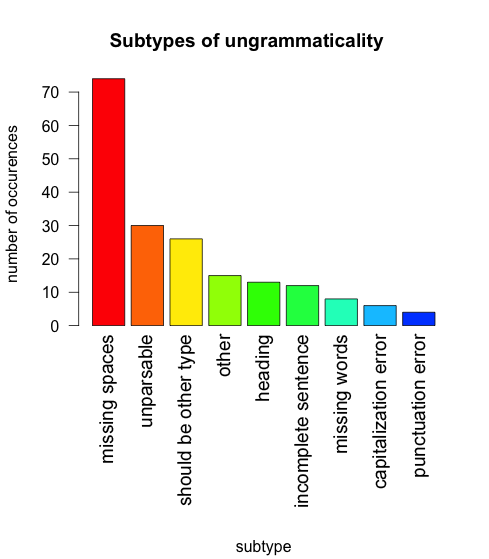
\includegraphics[scale=0.6]{subtypes_dev2.png}
\end{center}
\caption{\textbf{Subtypes of ungrammaticality in \textit{dev-2}.} Where the annotator didn't know what subtype to annotate the sentence with, they selected ``other''.}
\label{subtypes}
\end{figure}

\section{Experiments}
\label{experiments}
% All experiments, intermixed with small discussion segments
%TODO more intro
We conduct a number of experiments to find reliable ways to detect different kinds of ungrammaticality. The annotation, our experiments and the evaluation are all done on sentence basis. We use Stanford CoreNLP \citep{manning-EtAl:2014:P14-5} for sentence splitting.

\subsection{Detecting Ungrammaticality}
\label{sec_unknowntokens}
Perhaps the most noticeable result is the large portion of \textit{missing spaces} violations, meaning clauses that include tokens which aren't correct words. Almost all of these cases come from a missing space between two words forming tokens such as \texttt{reportsreaching} or \texttt{Wenchuancounty}. As there is such a large amount of this type, finding a reliable detection method for this subtype would significantly boost detection of ungrammaticality in general.

\subsubsection{The UnknownTokens method}
We call our straightforward approach to identifying missing spaces \textbf{UnknownTokens}: Tagging a sentence as containing a \textit{missing spaces} ungrammaticality if and only if there is a token in the sentence that isn't a ``known'' token, i.e. one that doesn't exist in a list of known words. In our setting, we can easily deduce such a list from the source documents of the automatic summarization process. If the source document is available and used as a base for our vocabulary, we call that approach \textbf{UnknownTokens\textsubscript{source}}.

In case the original documents aren't available or this method should be used in a different setting, we also investigate how to adapt our approach to that. This approach has a few steps, which we will all evaluate individually:
First, an initial list of words is created from a large text corpus (\textbf{UnknownTokens\textsubscript{gw}}); we use the first 20\% of the AFE part of the gigaword corpus \citep{gigaword}. If the corpus is large and general enough, this will probably cover a large vocabulary.

Because this will not include words for named entities yet, we only consider a token to be an unknown token, if it is not tagged as a Named Entity by a Named Entity Recognizer (\textbf{UnknownTokens\textsubscript{ner}}). We employ the Stanford Named Entity Recognizer \citep{stanfordNER}, which is a widely used, state-of-the-art NER that comes with a model for the English language.

In order to improve upon the NER and further increase recall, we use two simple heuristics (\textbf{UnknownTokens\textsubscript{heur}}): Firstly, we assume that words that start with a capital letter and are only followed by lower case letters are named entities and therefore no unknown tokens. Finally, we automatically check whether an unknown token has an entry on the online encyclopedia Wikipedia (\textbf{UnknownTokens\textsubscript{wiki}}).

We automatically label any tokens that are neither on our list of known tokens from GigaWord, nor tagged as a named entity as ``unknown'' and tag the sentence as containing unknown tokens. The combined method \textbf{UnknownTokens\textsubscript{gw+heur+ner+wiki}} is what we call \textbf{UnknownTokens\textsubscript{general}}.

\subsubsection{Evaluation of UnknownTokens}
We evaluate how effective \textbf{UnknownTokens} is in detecting \texttt{missing spaces} violations, both with (\textbf{UnknownTokens\textsubscript{source}}) and without (\textbf{UnknownTokens\textsubscript{general}}) access to the source documents, and compare it to a \textbf{baseline}, which always assumes the most common case (no \texttt{missing spaces} violation).
The standard metrics precision, recall and F-score are used for evaluation.

Table~\ref{eval_unknowntokens} shows the results of the evaluation. Because the amount of sentences not containing a missing spaces violation is much larger than the ones that do, several weighted metrics are provided, too:

The micro-average method consists of summing up the individual values from the confusion matrix (True Positive, False Positive, True Negative and False Negative) and calculating new metrics based on the results. We only display the F-score here, since F-score, recall and precision are identical for a 2-class scenario: Since the true positives of the missing spaces class are identical with the true negatives of the no missing spaces class (and vice versa), the new number of true positives and true negatives (for the micro average) is $tp + tn$ of any of the two classes. The same goes for false negatives and false positives. That means that when only dealing with two classes, in the micro-average method, the terms \textit{positive} and \textit{negative} can be used interchangeably. As precision is defined as $\frac{tp}{tp+fp}$ and recall as $\frac{tp}{tp+fn}$; as the equations only differ in whether they use $fp$ or $fn$ (which are exactly the same here) in the divisor, precision and recall (and therefore F-score, too, since the F-score is simply the harmonic mean of precision and recall) are identical.

Macro-averages are just arithmetic means of precision and recall. For both micro- and macro-average, the new F-score is calculated from the new scores.

Both \textbf{UnknownTokens\textsubscript{general}} and \textbf{UnknownTokens\textsubscript{source}} improve vastly over the baseline, but it is clear, that if the source text is available, it should be used to infer known words.


%%%BEGIN BACKUP WITHOUT WEIGHTED MEAN:
\begin{sidewaystable}
\begin{center}
\begin{tabular}{r|c|c|c|c|c|c|c|c|}
& \multicolumn{3}{c|}{Missing spaces} & \multicolumn{3}{c|}{No missing spaces} & Macro-average & Accuracy\\
& \textbf{P} & \textbf{R} & \textbf{F} & \textbf{P} & \textbf{R} & \textbf{F} & \textbf{F} & \\
\hline
\textbf{Baseline} & 0.0 & 0.0 & 0.0 & 94.8 & \textbf{100} & 97.3 & 48.7 & 94.8\\
\hline
\textbf{UT\textsubscript{gw}} & 15.0 & \textbf{98.7} & 26.0 & \textbf{99.9} & 69.1 & 81.7 & 68.2 & 70.7\\
\hline
\textbf{UT\textsubscript{gw+heur}} & 30.5 & 97.3 & 46.5 & 99.8 & 87.8 & 93.4 & 76.5 & 88.3\\
\hline
\textbf{UT\textsubscript{gw+heur+ner}} & 35.5 & 97.3 & 52.0 & 99.8 & 90.3 & 94.8 & 78.6 & 90.6\\
\hline
\textbf{UT\textsubscript{gw+heur+ner+wiki}} & 70.3 & 96.0 & 81.2 & 99.8 & 97.8 & 98.8 & 90.6 & 97.7\\
\hline
\textbf{UT\textsubscript{source}} & \textbf{95.9} & 94.6 & \textbf{95.2} & 99.7 & 99.7 & \textbf{99.7} & \textbf{97.5} & \textbf{99.5}\\
\end{tabular}
\end{center}
\caption{Evaluation of \textbf{UnknownTokens} on \textit{dev-2}, in percent. \textbf{UT\textsubscript{wordnet+heur+ner+wiki}} is equivalent to \textbf{UnknownTokens\textsubscript{general}}. \textbf{\textsubscript{wn}} = Wordnet-based dictionary, \textbf{\textsubscript{heur}} = title case heuristics, \textbf{\textsubscript{ner}} = Stanford NER, \textbf{\textsubscript{wiki}} = Wikipedia entry check}
\label{eval_unknowntokens}
\end{sidewaystable}
%%%END BACKUP WITHOUT WEIGHTED MEAN

%%%BACKUP WITH WEIGHTED MEAN:
% \begin{sidewaystable}
% \begin{center}
% \begin{tabular}{r|c|c|c|c|c|c|c|c|c|c|c|c|c|c|c|}
% & \multicolumn{3}{c|}{Positive Set} & \multicolumn{3}{c|}{Negative Set} & \multicolumn{3}{c|}{Weighted Mean} & Micro-average & \multicolumn{3}{c|}{Macro-average}\\
% & \textbf{P} & \textbf{R} & \textbf{F} & \textbf{P} & \textbf{R} & \textbf{F} & \textbf{P} & \textbf{R} & \textbf{F} & \textbf{F} & \textbf{P} & \textbf{R} & \textbf{F}\\
% \hline
% \textbf{Baseline} & 0.0 & 0.0 & 0.0 & 94.79 & 100 & 97.33 & 89.85 & 94.79 & 92.26 & 94.79 & 47.40 & 50.0 & 48.67\\
% \hline
% \textbf{UT\textsubscript{wn}} & 14.96 & 98.65 & 25.98 & 99.89 & 69.14 & 81.72 & 95.47 & 70.68 & 78.82 & 70.68 & 57.43 & 83.90 & 68.19\\
% \hline
% \textbf{UT\textsubscript{wn+heur}} & 30.51 & 97.30 & 46.45 & 99.83 & 87.81 & 93.43 & 96.22 & 88.30 & 90.98 & 88.30 & 65.17 & 92.56 & 76.49\\
% \hline
% \textbf{UT\textsubscript{wn+heur+ner}} & 35.47 & 97.30 & 51.99 & 99.84 & 90.26 & 94.81 & 96.49 & 90.63 & 92.58 & 90.63 & 67.66 & 93.78 & 78.61\\
% \hline
% \textbf{UT\textsubscript{wn+heur+ner+wiki}} & 70.30 & 95.95 & 81.15 & 99.77 & 97.77 & 98.76 & 98.23 & 97.68 & 97.84 & 97.67 & 85.04 & 96.86 & 90.57\\
% \hline
% \textbf{UT\textsubscript{source}} & 95.89 & 94.59 & 95.24 & 99.70 & 99.70 & 99.70 & 99.50 & 99.43 & 99.47 & 99.50 & 97.80 & 97.15 & 97.47\\


% \end{tabular}
% \end{center}
% \caption{Evaluation of \textbf{UnknownTokens} on \textit{dev-2}, in percent. \textbf{UT\textsubscript{wordnet+heur+ner+wiki}} is equivalent to \textbf{UnknownTokens\textsubscript{general}}. \textbf{\textsubscript{wn}} = Wordnet-based dictionary, \textbf{\textsubscript{heur}} = title case heuristics, \textbf{\textsubscript{ner}} = Stanford NER, \textbf{\textsubscript{wiki}} = Wikipedia entry check}
% \label{eval_unknowntokens}
% \end{sidewaystable}
%%%END BACKUP WITH WEIGHTED MEAN


\subsubsection{The RandomForest\textsubscript{UT} method}
% previous tries with LMs(?), unknown_tokens, unknown_tokens+LM+weka->decision trees
%TODO mention previous tries with LMS?
%TODO Tabelle
To detect more general forms of ungrammaticality, several other methods were investigated. Following \cite{wagner2007comparative}, we learn decision trees from outputs of several systems that on their own have not proven sufficient for this task. For this experiment, the development set \textit{dev-1} was used.

We train a language model on parts (the same parts we used as a word source in \textbf{UnknownTokens\textsubscript{general}} (section~\ref{sec_unknowntokens})) of the Gigaword corpus\citep{gigaword}, extract perplexity scores for the sentences in our test set, and annotate them automatically. For the language model generation and the extraction of perplexity scores, we employ SRILM~\citep{stolcke2002srilm}, a language modeling toolkit.


%The free WEKA software~\citep{hall2009weka} is an allround machine learning toolkit.
We then use a RandomForest \citep{breiman2001random} to learn decision trees. For this task, we use the machine learning toolkit WEKA \citep{hall2009weka}.
%As an input, WEKA requires an ARFF file, which we created using three features:
We use three features for our decision tree:

\begin{itemize}
	\item \textbf{LM\_PP} is the perplexity calculated for a sentence by the language model, following \cite{sun2007detecting}. This is a numeric feature. It proved to not be sufficient for detecting ungrammaticality on its own.
	\item \textbf{missing spaces} is the classification of \textbf{UnknownTokens\textsubscript{source}} for a given sentence, as described in section~\ref{sec_unknowntokens}. This is a binary feature.
	\item \textbf{numberofwords} is the number of words in the sentence. We follow \cite{wagner2007comparative} here, the intuition is that ungrammatical sentences will often be extraordinarily long, or very short:

		\textit{Former US President George W Bush, Who Will attend a memorial service on Tuesday, Virginia, and the university of at least 33 people Were killed, in the Worst shooting rampage in modern history, the White House said.}

		\textit{The report of a}
\end{itemize}

\subsubsection{Evaluation of RandomForest\textsubscript{UT}}
\label{S_eval_randomforest}

We performed 10-fold cross-validation, which lead to a weighted F-score of 86.3\%. A total of 1215 (88.1\%) instances was classified correctly, 164 (11.9\%) incorrectly.

% === Run information ===

% Scheme:       weka.classifiers.trees.RandomForest -I 10 -K 0 -S 1 -num-slots 1
% Relation:     ungrammaticality
% Instances:    1379
% Attributes:   4
%               language_model
%               nonwords
%               numberofwords
%               class
% Test mode:    10-fold cross-validation

% === Classifier model (full training set) ===

% Random forest of 10 trees, each constructed while considering 3 random features.
% Out of bag error: 0.1291



% Time taken to build model: 0.43 seconds

% === Stratified cross-validation ===
% === Summary ===

% Correctly Classified Instances        1215               88.1073 %
% Incorrectly Classified Instances       164               11.8927 %
% Kappa statistic                          0.3351
% Mean absolute error                      0.1491
% Root mean squared error                  0.3094
% Relative absolute error                 65.2325 %
% Root relative squared error             91.6119 %
% Coverage of cases (0.95 level)          96.2292 %
% Mean rel. region size (0.95 level)      66.4612 %
% Total Number of Instances             1379     

% === Detailed Accuracy By Class ===

%                  TP Rate  FP Rate  Precision  Recall   F-Measure  MCC      ROC Area  PRC Area  Class
%                  0.970    0.707    0.901      0.970    0.934      0.361    0.766     0.938     ungrammaticality-no
%                  0.293    0.030    0.596      0.293    0.393      0.361    0.766     0.417     ungrammaticality-yes
% Weighted Avg.    0.881    0.618    0.861      0.881    0.863      0.361    0.766     0.869     

% === Confusion Matrix ===

%     a    b   <-- classified as
%  1162   36 |    a = ungrammaticality-no
%   128   53 |    b = ungrammaticality-yes

\subsubsection{The RandomForest\textsubscript{parser} method}
We also investigated whether parser output would improve the results. For this task, we utilized the Answer Constraint Engine \citep{ace} with the English Resource Grammar \citep{copestake2002implementing} to parse the entire corpus and annotate it with output statistics of the parser: Following \cite{wagner2007comparative} loosely, we extracted the number of readings/parses, the amount of memory the parser used for the parse and the success status, which could be either ``ok'' or ``ignored'', the latter appearing when the parsing failed entirely for some reason.

We then added these three features to \textbf{RandomForest\textsubscript{UT}}.

\subsubsection{Evaluation of RandomForest\textsubscript{parser}}

When evaluating the emerging decision tree on general ungrammaticality using the same method as in Section~\ref{S_eval_randomforest}, it yielded worse results than \textbf{RandomForest\textsubscript{UT}} alone. We therefore inspected whether it could instead be used to find instances of the subtype \textit{unparsable}. This lead to a precision of 86.6\%, a recall of 87.9\%, and an F-Score of 86.3\%. A total of 87.9\% of the instances was classified correctly.

\subsection{Datelines}
%TODO more examples (see defense.tex).
Source texts from news articles, like the ones in the TAC dataset, often contain datelines, which sometimes make it into the generated summary. While in the context of the article datelines made sense (often displayed smaller or otherwise visually distinctive), they are not needed, distracting and confusing in the summaries:

\textit{\textbf{BLACKSBURG, Virginia 2007-04-16 18:34: 44 UTC} A gunman opened fire in a dorm and classroom at Virginia Tech on Monday, killing at least 30 people in the deadliest shooting rampage in U.S. history.}



\subsubsection{Method}
The emerging patterns are so regular, that we use regular expressions to detect them. A few iterations of the regex were done, but so far the highest results were achieved using the regular expression

\begin{lstlisting}
UTC|^\d{4}-\d{2}-\d{2}|^[A-Z]{3,}|^(Jan|Feb|Mar|Apr|May|Jun|Jul|Aug|Sep|Oct|Nov|Dec)
\end{lstlisting}

The expression has four parts, of which only one has to match to make the system classify a sentence as containing datelines: The first part matches the string ``UTC'' (Coordinated Universal Time, a common fragment in datelines), the second one numeric dates like \texttt{2014-04-13}, the third one capitalized words that are longer than 4 letters and are therefore expected not to be abbreviations (an example would be \texttt{LONDON, Feb. 4 (Xinhua)}), and the final part matches abbreviated names of months. Only ``UTC'' can occur anywhere, everything else needs to occur at the beginning of a sentence to be counted.

\subsubsection{Evaluation}
This very simple approach was evaluated on \textit{dev-2} and leads to good results: The F-score of the class of dateline-containing sentences is 90.7\% (precision: 90.3\%, recall: 91.1\%). When looking into the inaccurately detected instances, the inconsistencies of the LQVSumm corpus make up most of the misses:

%PRF = 86.0\% & 89.7\% & 87.8\%\\ %TODO on test-345

\textit{IVORY TUSKS}

is classified as containing a dateline by the regular expression, but is not annotated as such in the corpus. An example of a false negative would be:

\textit{00 a.m. local time (0800 GMT)}

which our system doesn't match.

\subsection{Redundancy}
\label{redundancy}
% token overlap
% threshold auf dev-Set perfekt machen, auf test-set testen
% gegen Ende: wordnet most-frequent-sense
%TODO other experiments?

Automatic summaries constructed from multiple source texts on the same topic often suffer from redundancy, as sentences that contain the same or largely the same information are occasionally included in the summary. As a consequence, reading fluency is impaired.

While --- in contrast to many other linguistic quality violations --- this also has an impact on traditional evaluation scores for automatic summarization systems (because the information density is lower than it could be), it is also considered to be a problem of our domain.

In the LQVSumm corpus, different degrees of redundant sentence pairs occur. Some sentence pairs annotated as redundant contain similar information, but using completely different phrasing and focus:

%low example
\textit{According to a survey by the State Food and Drug Administration, 65 percent of the respondents worried about the food safety situation in China.}

\textit{Food and drug safety has become a major concern of Chinese people.}

Other pairs of sentences are apparently at least partly composed of the same source sentence, but are still different. One of the sentences might contain additional information and the two sentences might still be of very different length:

%medium example
\textit{Cyclone Sidr, described as the worst storm in years to hit low-lying and disaster-prone Bangladesh, crashed into the southwestern coast Thursday night before sweeping north over the capital Dhaka.}

\textit{The cyclone hit the southwestern coast of Bangladesh on Thursday before sweeping north to the capital Dhaka.}

Finally, sometimes subsequent sentences have marginal differences:
%high example
\textit{An unknown number of cats and dogs suffered kidney failure and about 10 died after eating the affected pet food, Menu Foods said in announcing the North American recall.}

\textit{An unknown number of cats and dogs suffered kidney failure, and about 10 died after eating the affected pet food, Menu Foods said in announcing the North American recall.}

We are seeking to find all of these sentences, but concentrate on the latter two cases where the redundancy is obvious for humans.

\subsubsection{Method}
%TODO bigrams stemmed vs. unstemmed in table?

Our method (\textbf{Unigrams}) consists of a simple unigram overlap score, which we found to outperform more sophisticated approaches:

First, we remove all non-alphanumeric characters from both sentences and split them into words. We then treat the words as a set and divide the cardinality of the intersection of each sentence's set by the number of words in the smaller sentence. A given threshold is then used to classify instances.

A number of other methods are also implemented: \textbf{Bigrams} is a variation of the \textbf{Unigrams} method which uses bigrams instead of unigrams. \textbf{Combined} is using a score that the mean of the \textbf{Unigrams} and \textbf{Bigrams} scores.

\textbf{Levenshtein} consists of the standard edit distance\citep{levenshtein1966binary} on word level. A threshold of 2 yielded best results on our development set, meaning that sentences are classified as containing redundancies if their word-level Levenshtein distance is 1 or 0. Prior to computation of the score, non-alphanumeric characters were again pruned from the sentences.

Finally, as a further \textbf{Baseline} we classify all sentence pairs as containing redundancies.

We briefly considered using BLEU scores \citep{papineni2002bleu} for redundancy detection (with the rationale that if the second sentence is a ``good translation'' of the first one, it might be redundant), but BLEU scores get their performance from having multiple reference translations available, which is not the case here.

\subsubsection{Evaluation}

In the corpus, redundancy isn't annotated on sentence base, but rather on clause level, where ``clause'' is an arbitrary substring of the summary text. That means that redundancy annotations can span over many sentences, can skip sentences inbetween and can be contained in a single sentence.

For our purposes, we only consider redundancies that occur in two subsequent sentences and our evaluation metrics are based on those.

To obtain a good threshold for \textbf{Unigrams}, \textbf{Bigrams}, and \textbf{Combined}, we compare their performance on the development sets \textit{dev-1} and \textit{dev-2}. The results can be seen in Figure~\ref{redundancy_graph}.

\begin{figure}
\begin{center}
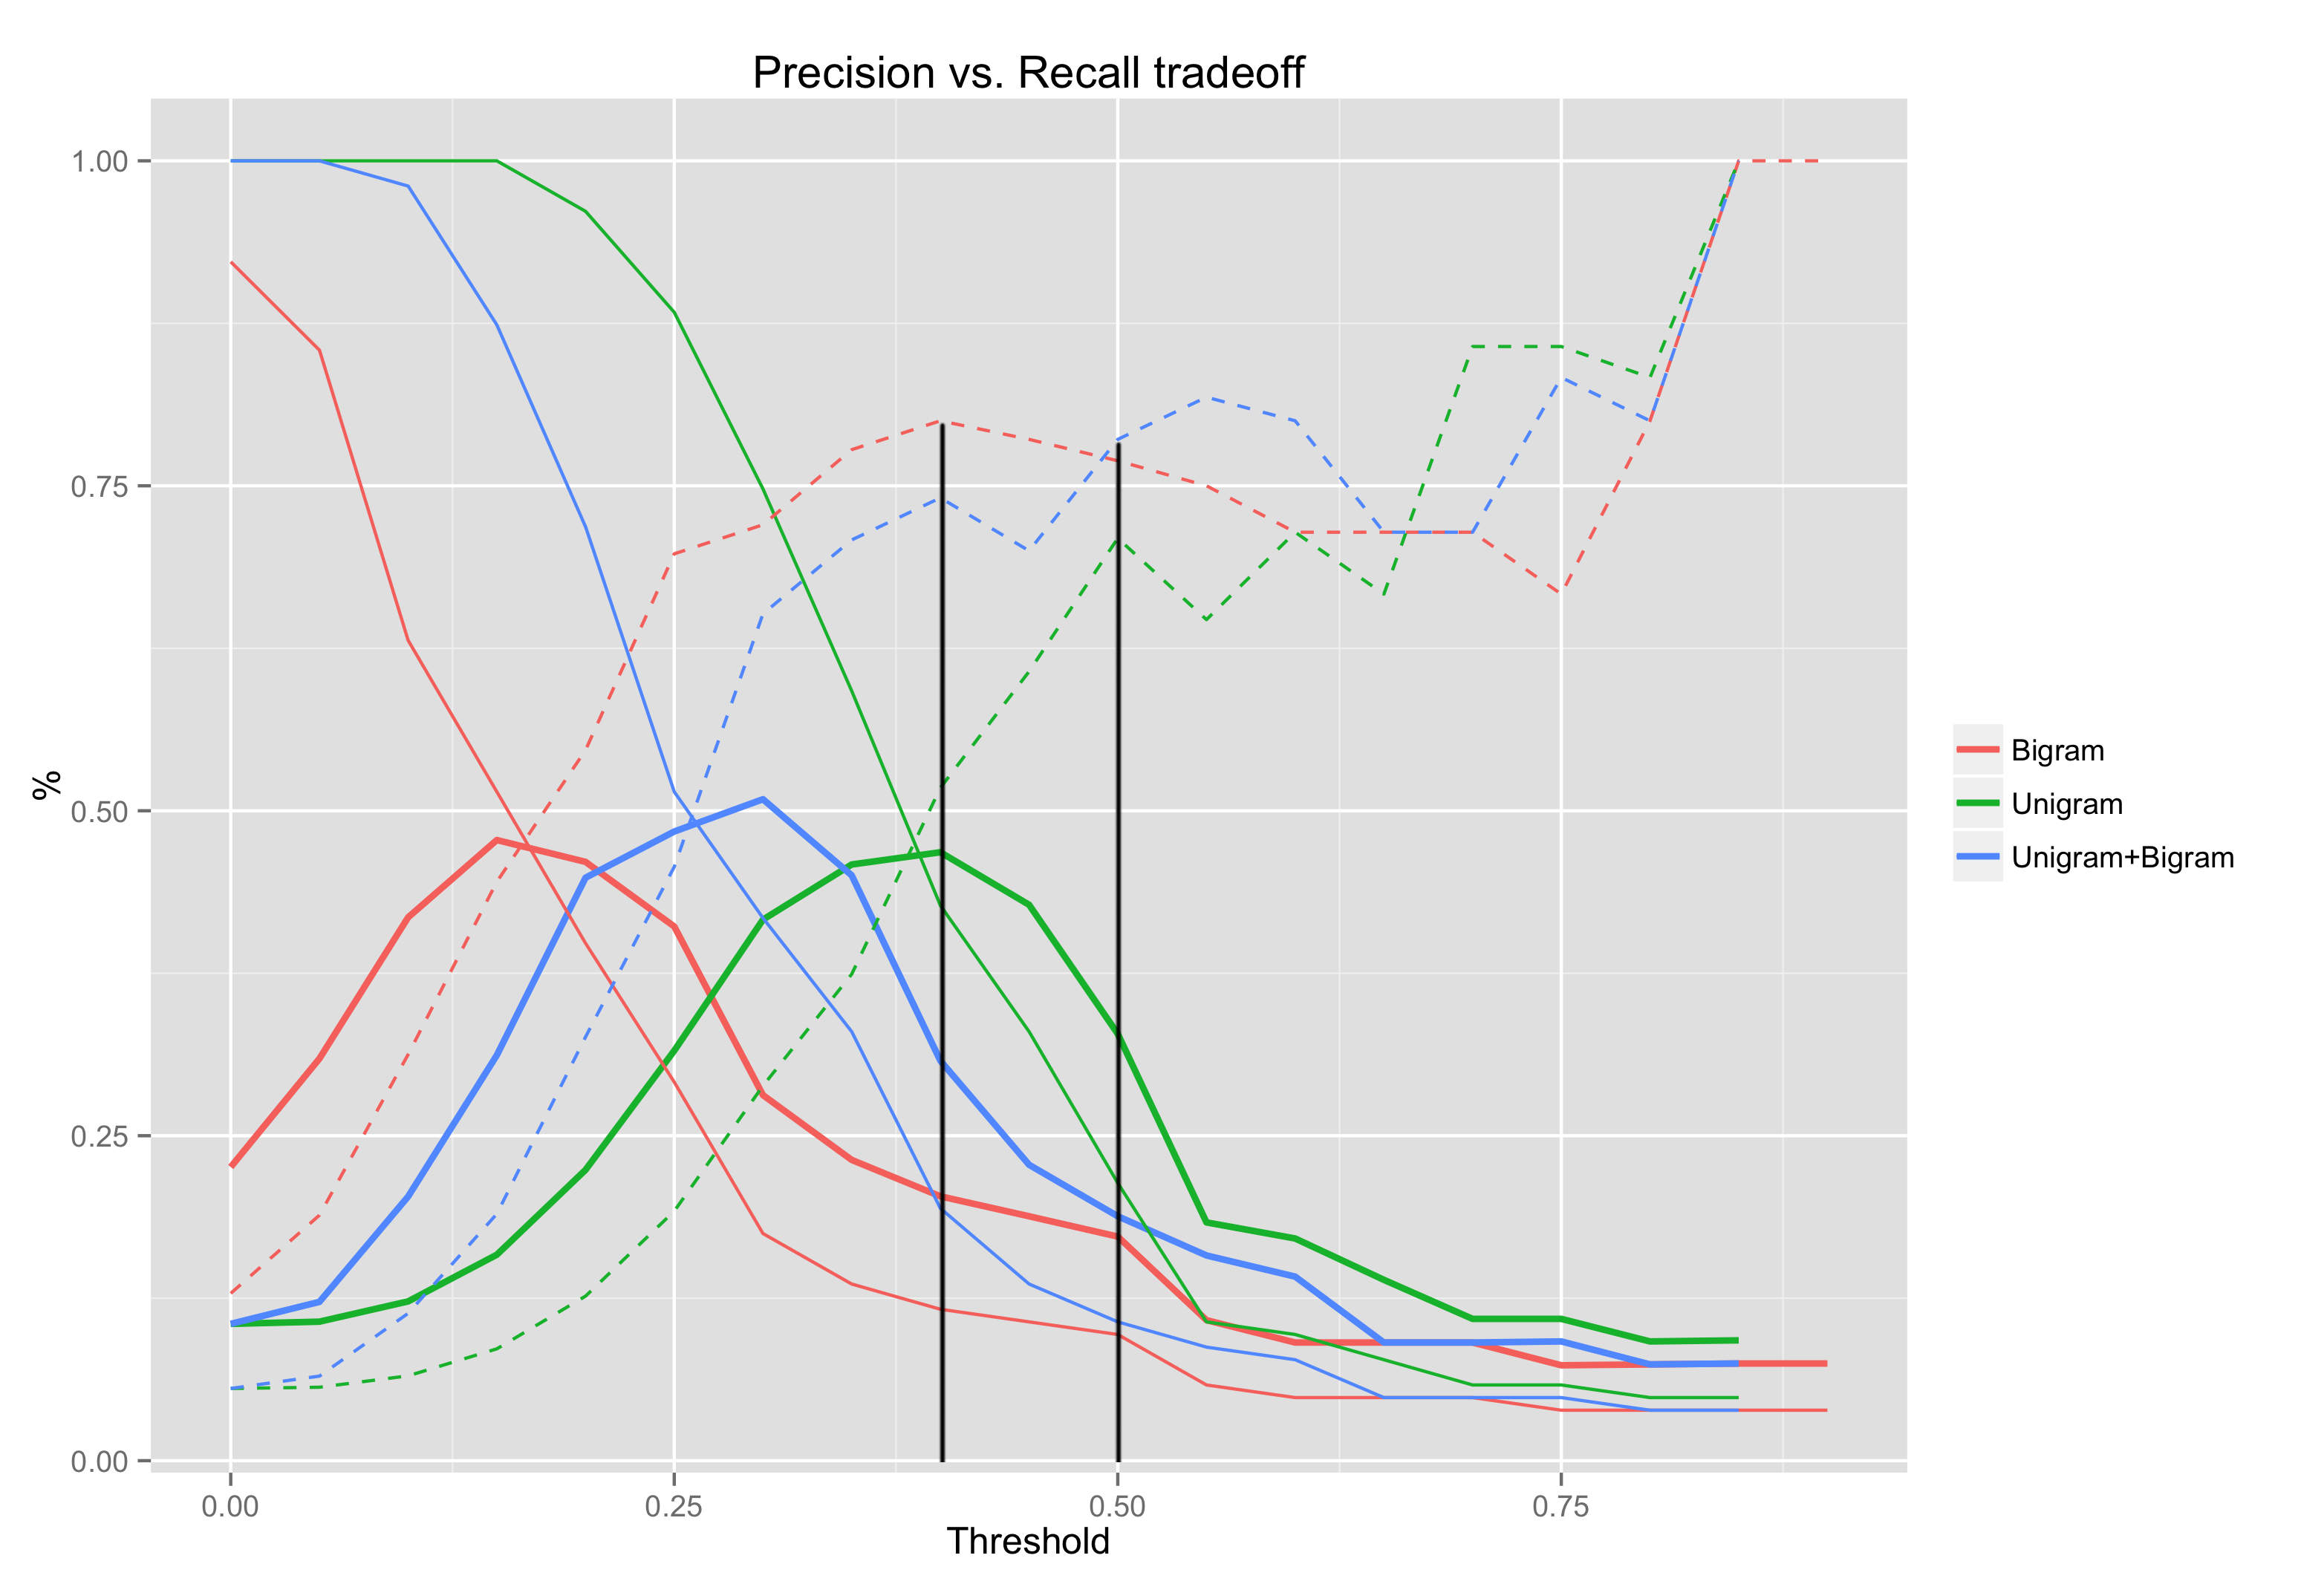
\includegraphics[scale=0.15]{a.png}
\end{center}
\caption{Performance of various thresholds for \textbf{Unigrams}, \textbf{Bigrams}, and \textbf{Combined} in \textit{dev-1} and \textit{dev-2}. Continuous lines are recall, dashed lines are precision and bold lines are F-score.}
\label{redundancy_graph}
\end{figure}

For recall, \textbf{Unigrams} outperforms \textbf{Bigrams}, while for precision \textbf{Bigrams} is predominant.

As is to be expected, higher thresholds correlate with higher precision and lower recall. And while the F-scores are given in Figure~\ref{redundancy_graph} for informational purposes, they are not what we want to optimize; while recall is desirable, we feel that precision is much more important for a system that annotates violations.

We therefore choose a threshold of $0.4$ for the \textbf{Bigrams} and \textbf{Combined}, and one of $0.5$ for \textbf{Unigrams}, because there appear to be local maxima at that point with still some amount of recall.

The results can be seen in Table~\ref{eval_redundancy}. Evidently, the \textbf{Unigrams} method outperforms \textbf{Levenshtein} and the \textbf{Baseline} as well as the other n-gram methods.

\begin{table}
\begin{center}
\begin{tabular}{r|c|c|c|}
& Precision & Recall & F-Score \\
\hline
\textbf{Baseline} & 4.5\% & \textbf{100\%} & 8.7\% \\
\hline
\textbf{Levenshtein} & 15.8\% & 17.3\% & 3.1\% \\
\hline
\textbf{Unigrams} & \textbf{58.0\%} & 28.2\% & \textbf{37.0\%} \\
\hline
\textbf{Bigrams} & 55.6\% & 14.5\% & 22.9\% \\
\hline
\textbf{Combined} & 56.8\% & 24.3\% & 34.0\% \\
\hline
\end{tabular}
\end{center}
\caption{Evaluation of \textbf{Unigrams}, \textbf{Bigrams}, and \textbf{Combined} on everything but \textit{dev-1} and \textit{dev-2}}
\label{eval_redundancy}
\end{table}

% Bigrams: 0.5555555555555556,0.14450867052023122,0.22935779816513763
% Combined: 0.5675675675675675,0.24277456647398843,0.340080971659919
% Unigrams: 0.5802469135802469,0.27167630057803466,0.3700787401574803

% Levenshtein: 0.15789473684210526,0.017341040462427744,0.03125

% Baseline: 0.045240585774058575,1.0,0.08656492369276958

%\subsection{Unrelatedness} %evtl %NOOO
%\section{Evaluation} oder auch nicht
% or skip entirely and put in experiments? final results here?

\section{Discussion}
\label{discussion}
% What seem to be the best methods for the various tasks and why?
% TODO Why does what works work and not that which doesn't? inkl examples !!
Detecting linguistic quality violations automatically is not a trivial task. It is not always easy for humans to produce consistent annotations and annotations aren't necessarily highly consistent across humans, as can be seen in the inter-annotator agreement in \cite{friedrichlqvsumm}.

Sometimes, however, the easier methods outperformed the more sophisticated approaches. This can be the case because...

%TODO einzelne Experimente..

%TODO mehr KRITIK!!
%TODO: no.
The corpus we used was not an optimal choice either.

The LQVSumm corpus that we used for all of our experiments is, unfortunately, not large enough to have a wide coverage of all violations. This can be seen most prominently when trying to detect redundancy (Section~\ref{redundancy}).

%TODO inappropriate->challenges
Apart from its size, the corpus is also often annotated inconsistently or at least inappropriate for our purposes. In general, annotations are done on the clause level, where clauses are arbitrary substrings of the summary. As we classify and evaluate on sentences produced by Stanford CoreNLP \citep{manning-EtAl:2014:P14-5}, this introduces noise.

Annotations aren't done consistently throughout the corpus, and often very different violations are annotated with the same label, the most obvious example of this being shown in Section~\ref{corpus_study}. This is not automatically a weakness of the corpus itself, but rather an unfitness for our purposes.
%TODO besser wenn vorher segmentierung (vor annotation), problem annotation vs automatic

%show example
However, there's little to no alternatives available.

A legitimate criticism of our work is that our methods, experiments, and results are tailored to the LQVSumm corpus or to the summarization systems that participated in the TAC 2011 Guided Summarization task \citep{owczarzak2011overview}.

%TODO what could be done better?


\section{Conclusion} % & Future Work
\label{conclusion}
% TODO What can my results be used for? What should be investigated later?
% TODO What could possibly be needed to work on the types not looked at here? (semrel, …)
%TODO other genres

In this paper, we have presented a solid method to detect the kind of ungrammaticality that occurs in automatically generated extractive multi-document summarizations. While the results are good, they do rely on a certain type of ungrammaticality occuring often (missing spaces). Future work could concentrate on improving other grammaticality violations, so that not only the accuracy rises, but also the generality. Such a system could potentially detect ungrammaticality in a much broader domain.

We have also shown a simple but high-performing method of detecting datelines. We believe our results are close to what a human could achieve and don't see much room for improvement here.

Finally we developed a basic method of detecting redundancy. With the lowest performance of all methods in this paper, redundancy detection is requiring much more work. While we based our approach only on the two subsequent sentences on which redundancy was to be tested, future work could include information available in the context of these sentences or even, as we did in \textbf{UnknownTokens\textsubscript{source}}, information from the source documents.

We only looked at a part of the violation types in \cite{friedrichlqvsumm}. Methods for detecting the last clause-level violation (no semantic relation), as well as the entity- and discourse-level violations have yet to be developed.

For the entity-level violations, one could use the output of a coreference resolution tool such as BART \citep{versley2008bart} or the Stanford coreference resolution system \citep{lee2011stanford} to infer coreferences between entities in the summaries as well as the source documents and compare the originating coreference chains.

Along with this paper, the authors will provide a toolchain that can be used to annotate given documents with the methods described in here.

\section*{Acknowledgments}

?
%Annemarie Friedrich
%Manfred Pinkal, Alexis Palmer
%Lukas Burk, Diana Asimi(?)

\newpage
\bibliographystyle{apalike}
\bibliography{referenzen}

\end{document}